\section{End-to-end Evaluation}
\label{sec:eval}

\noindent
We conclude our study of efficient LLM scheduling
by comparing {\sys} with the multiplication method described in {\textsection{\ref{sec:method}}}
and state-of-the-art schedulers on end-to-end LLM serving performance.

\begin{figure}[!t]
    \centering
    \begin{subfigure}{\linewidth}
        \centering
        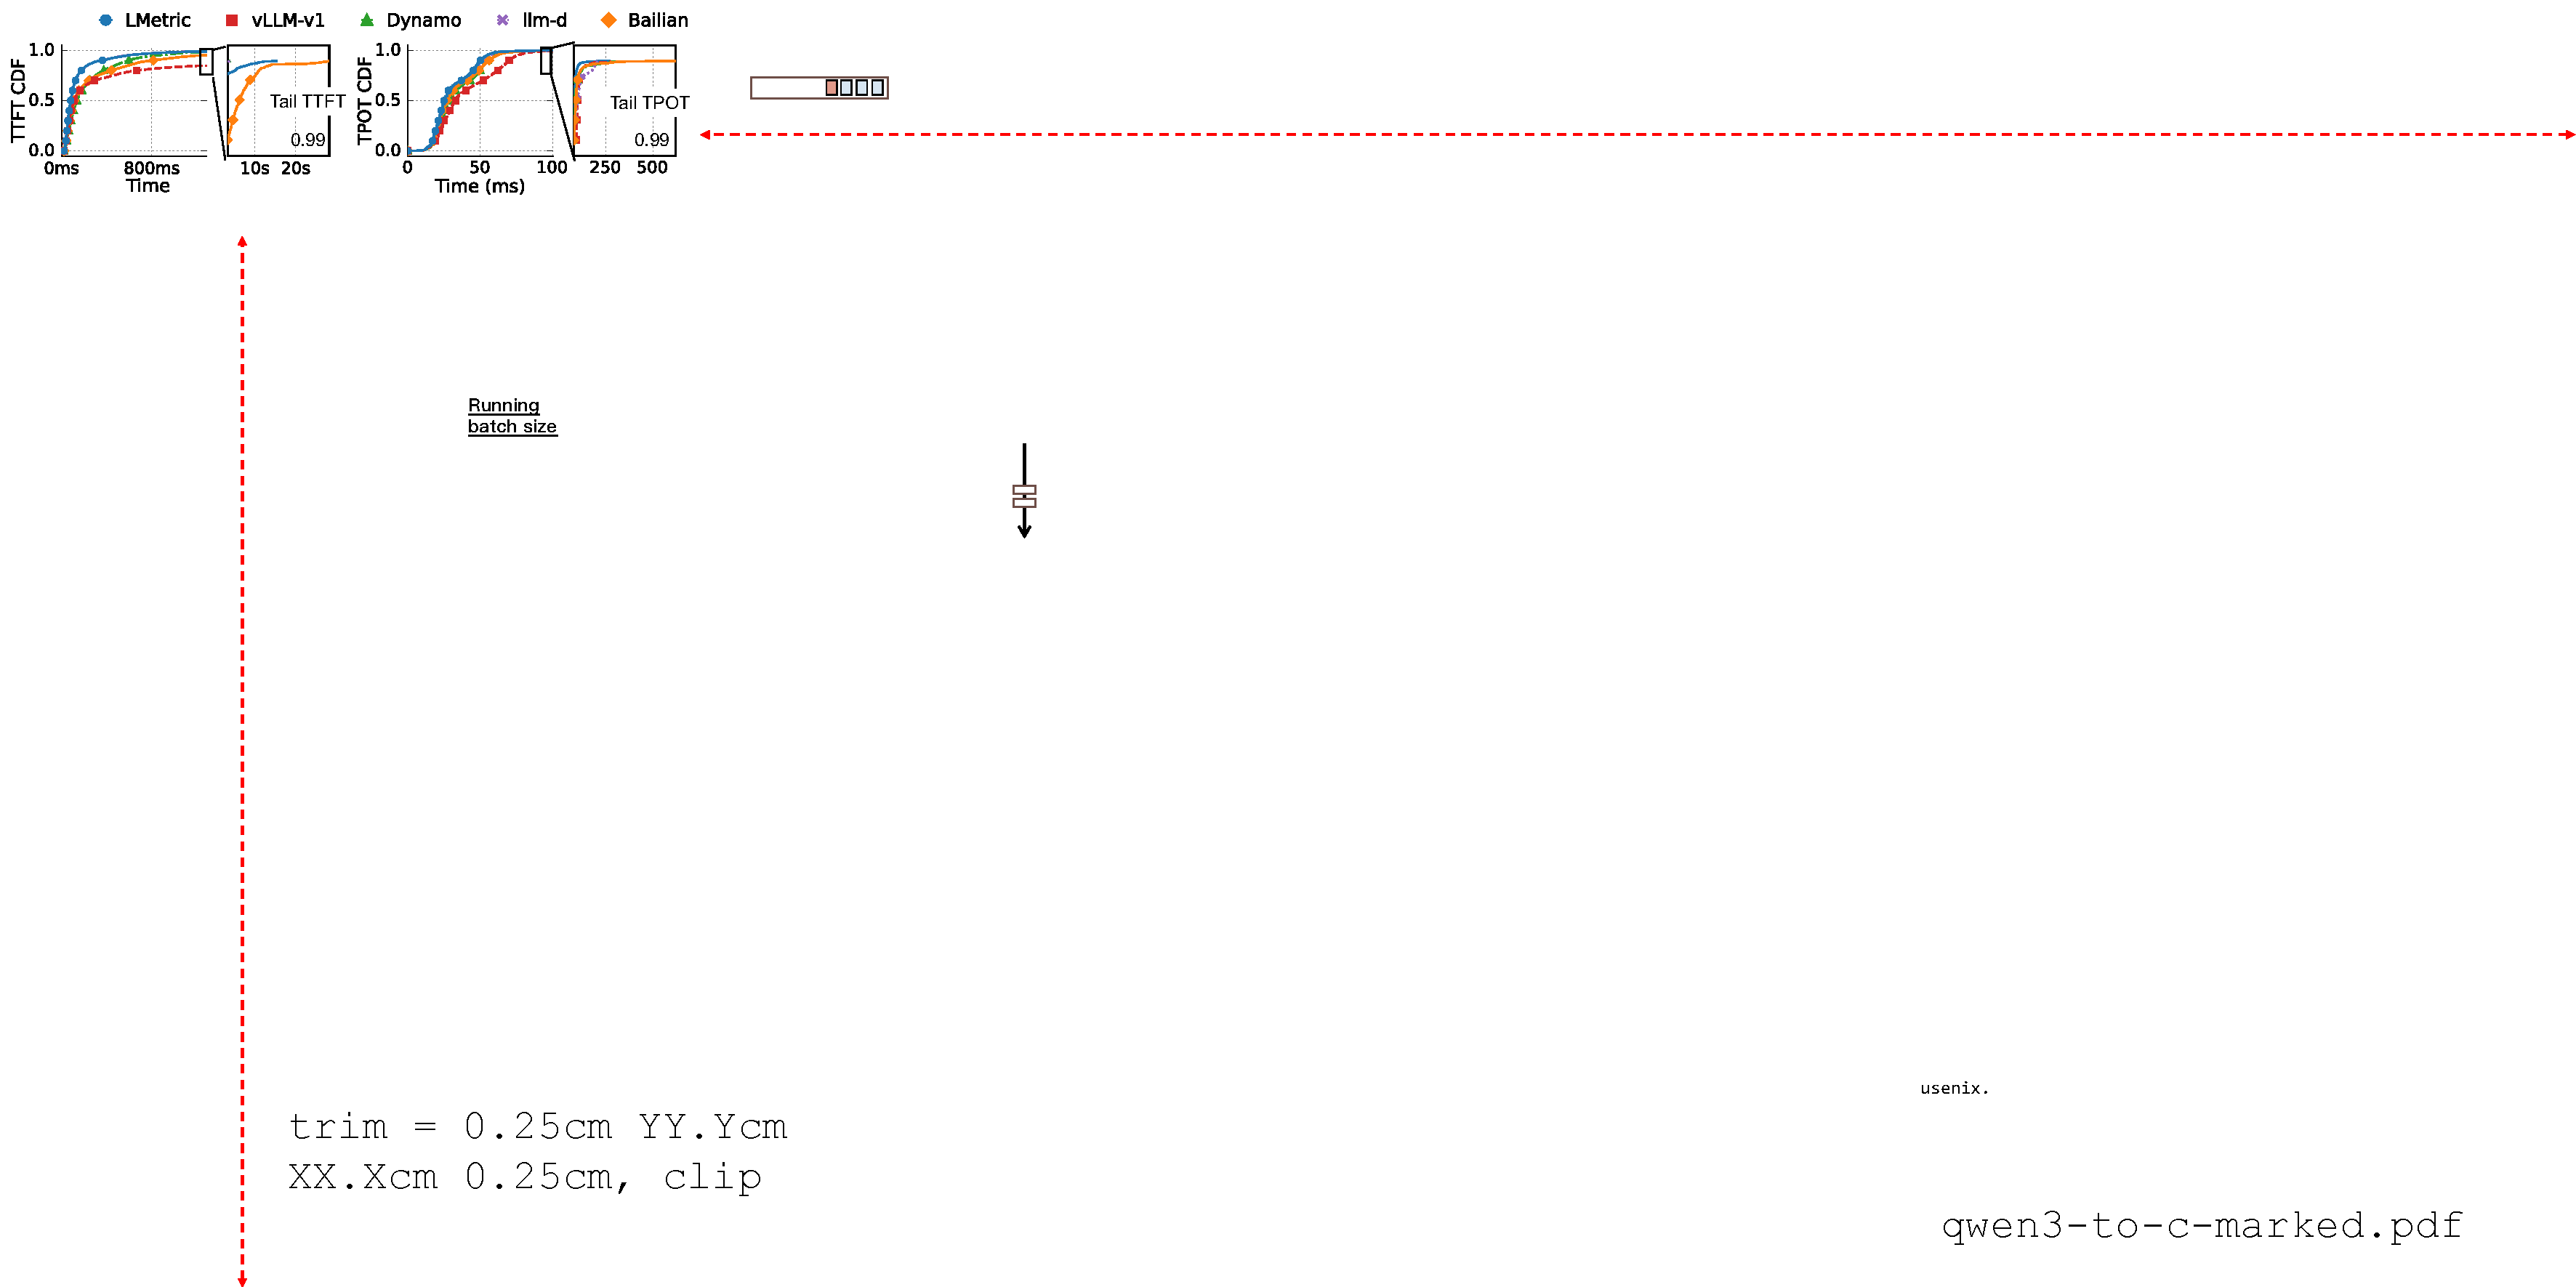
\includegraphics[width=0.98\linewidth, trim=0.25cm 25.2cm 43.75cm 0.25cm, clip]{figs/e2e-cdf-v1/qwen3-to-c-marked.pdf}
        \vspace{-8pt}
        \caption{\small{Qwen3-30B on ChatBot (Qwen) workload.}}
        \label{fig:eval-qwen3-to-c}
    \end{subfigure} \\[6pt]
    \begin{subfigure}{\linewidth}
        \centering
        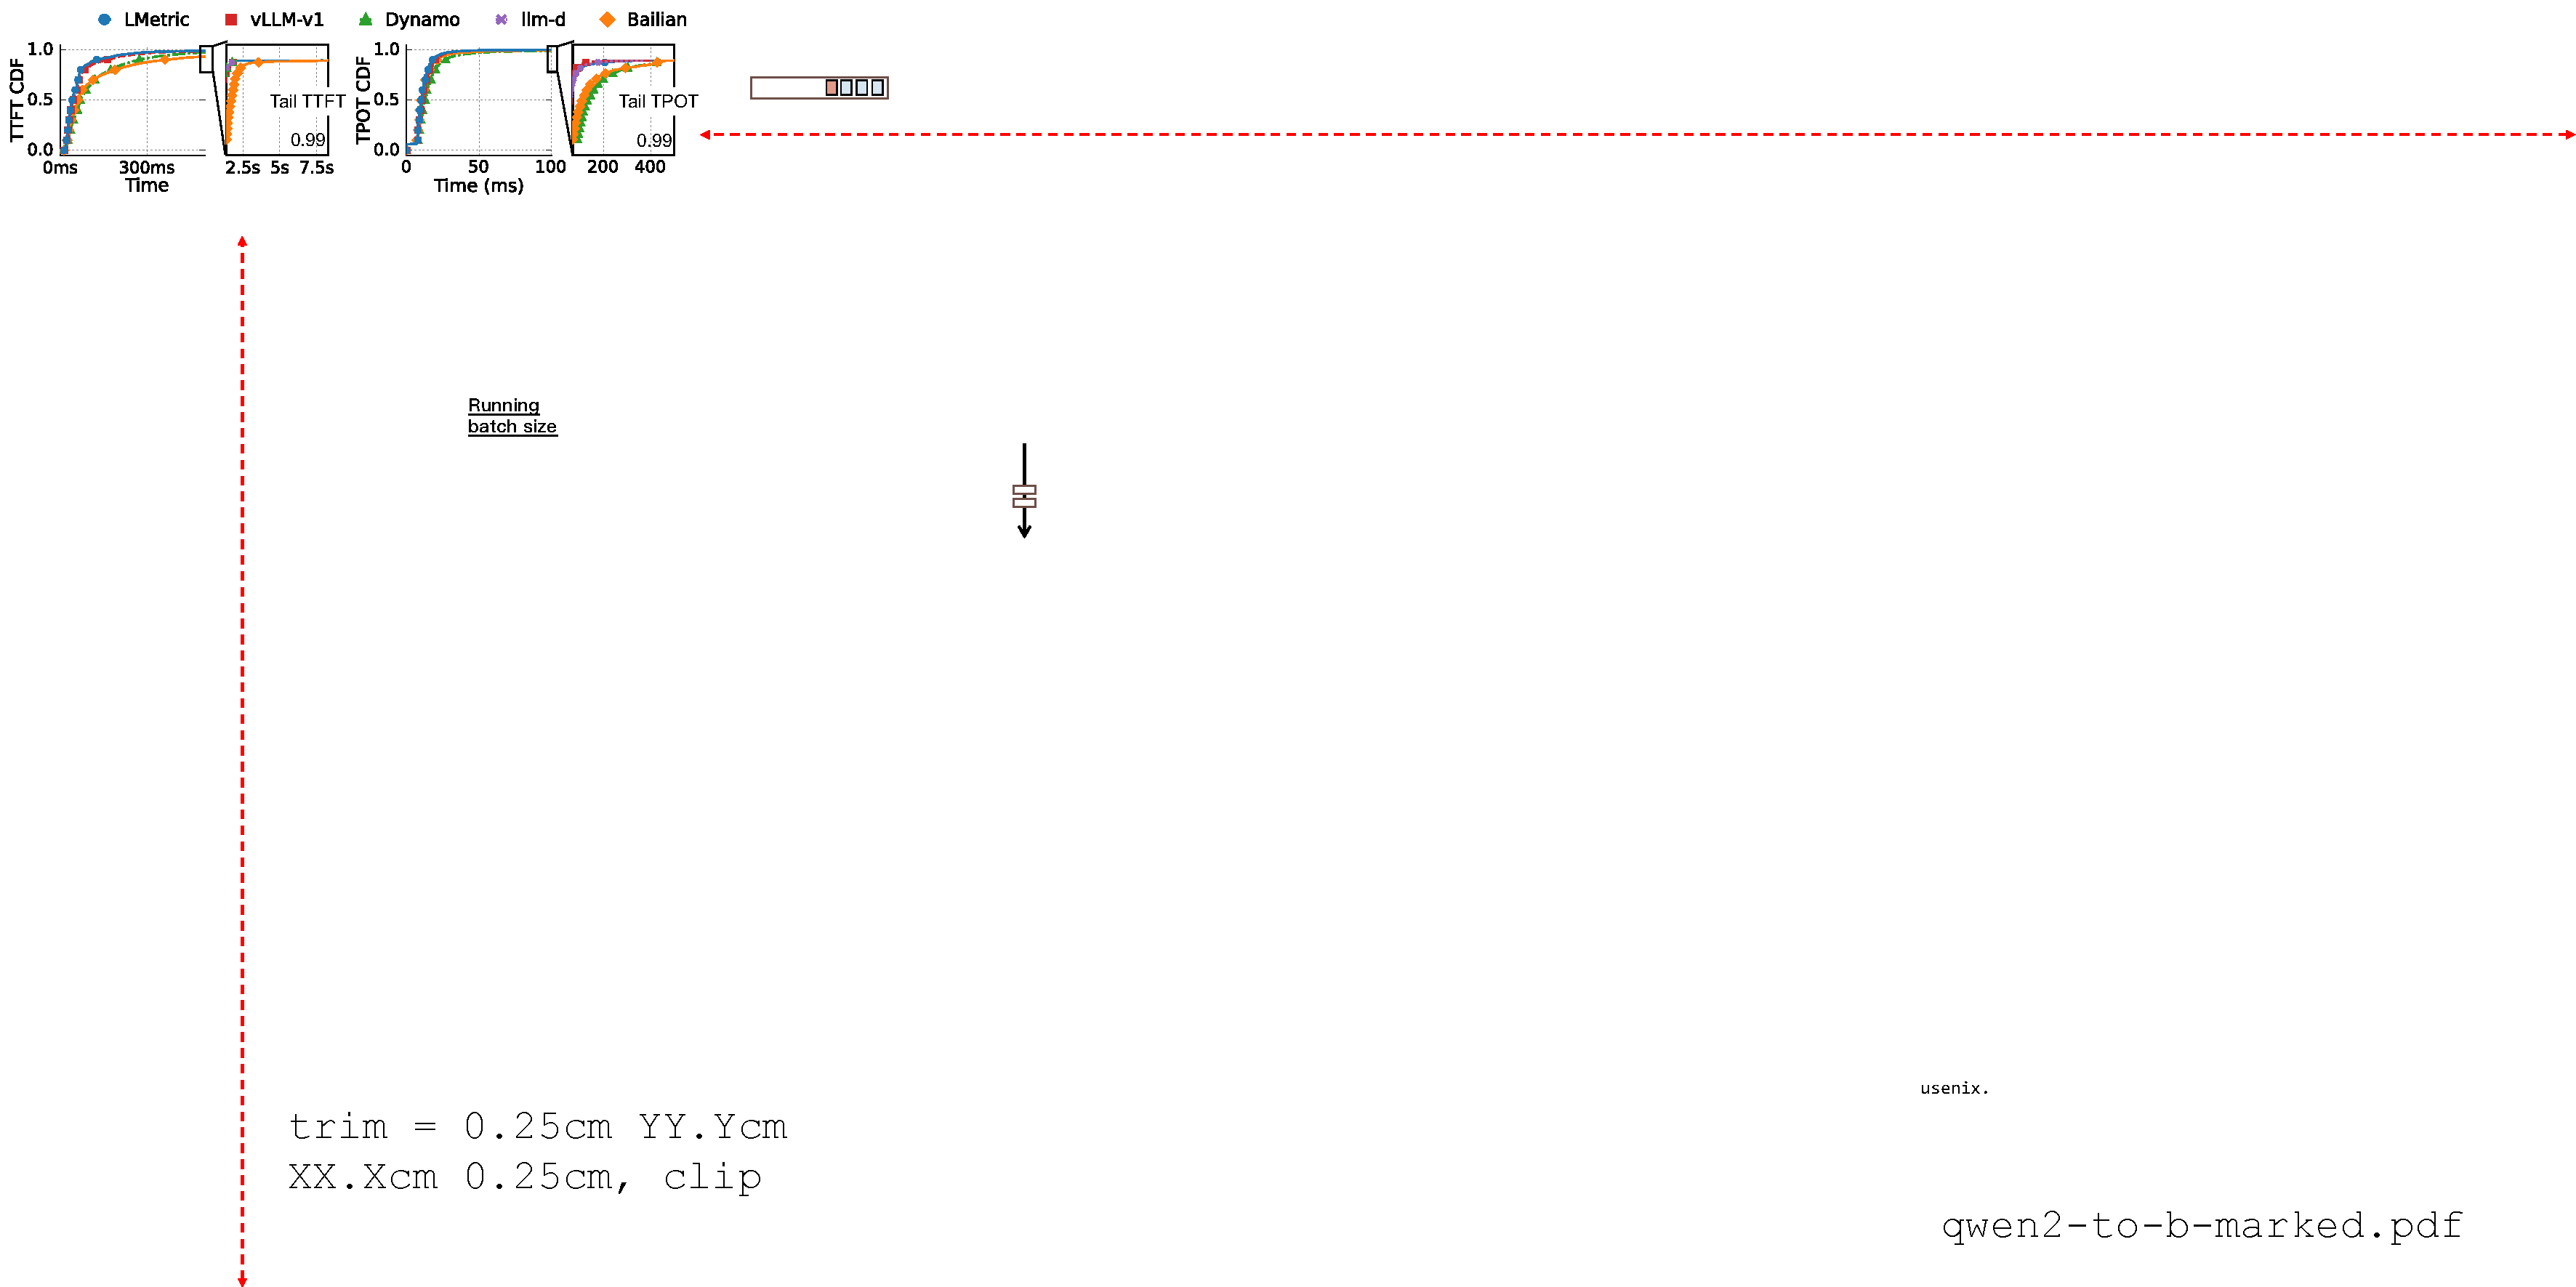
\includegraphics[width=0.98\linewidth, trim=0.25cm 25.2cm 43.75cm 0.25cm, clip]{figs/e2e-cdf-v1/qwen2-to-b-marked.pdf}
        \vspace{-8pt}
        \caption{\small{Qwen2-7B on Agent (Qwen) workload.}}
        \label{fig:eval-qwen2-to-b}
    \end{subfigure} \\[6pt]
    \begin{subfigure}{\linewidth}
        \centering
        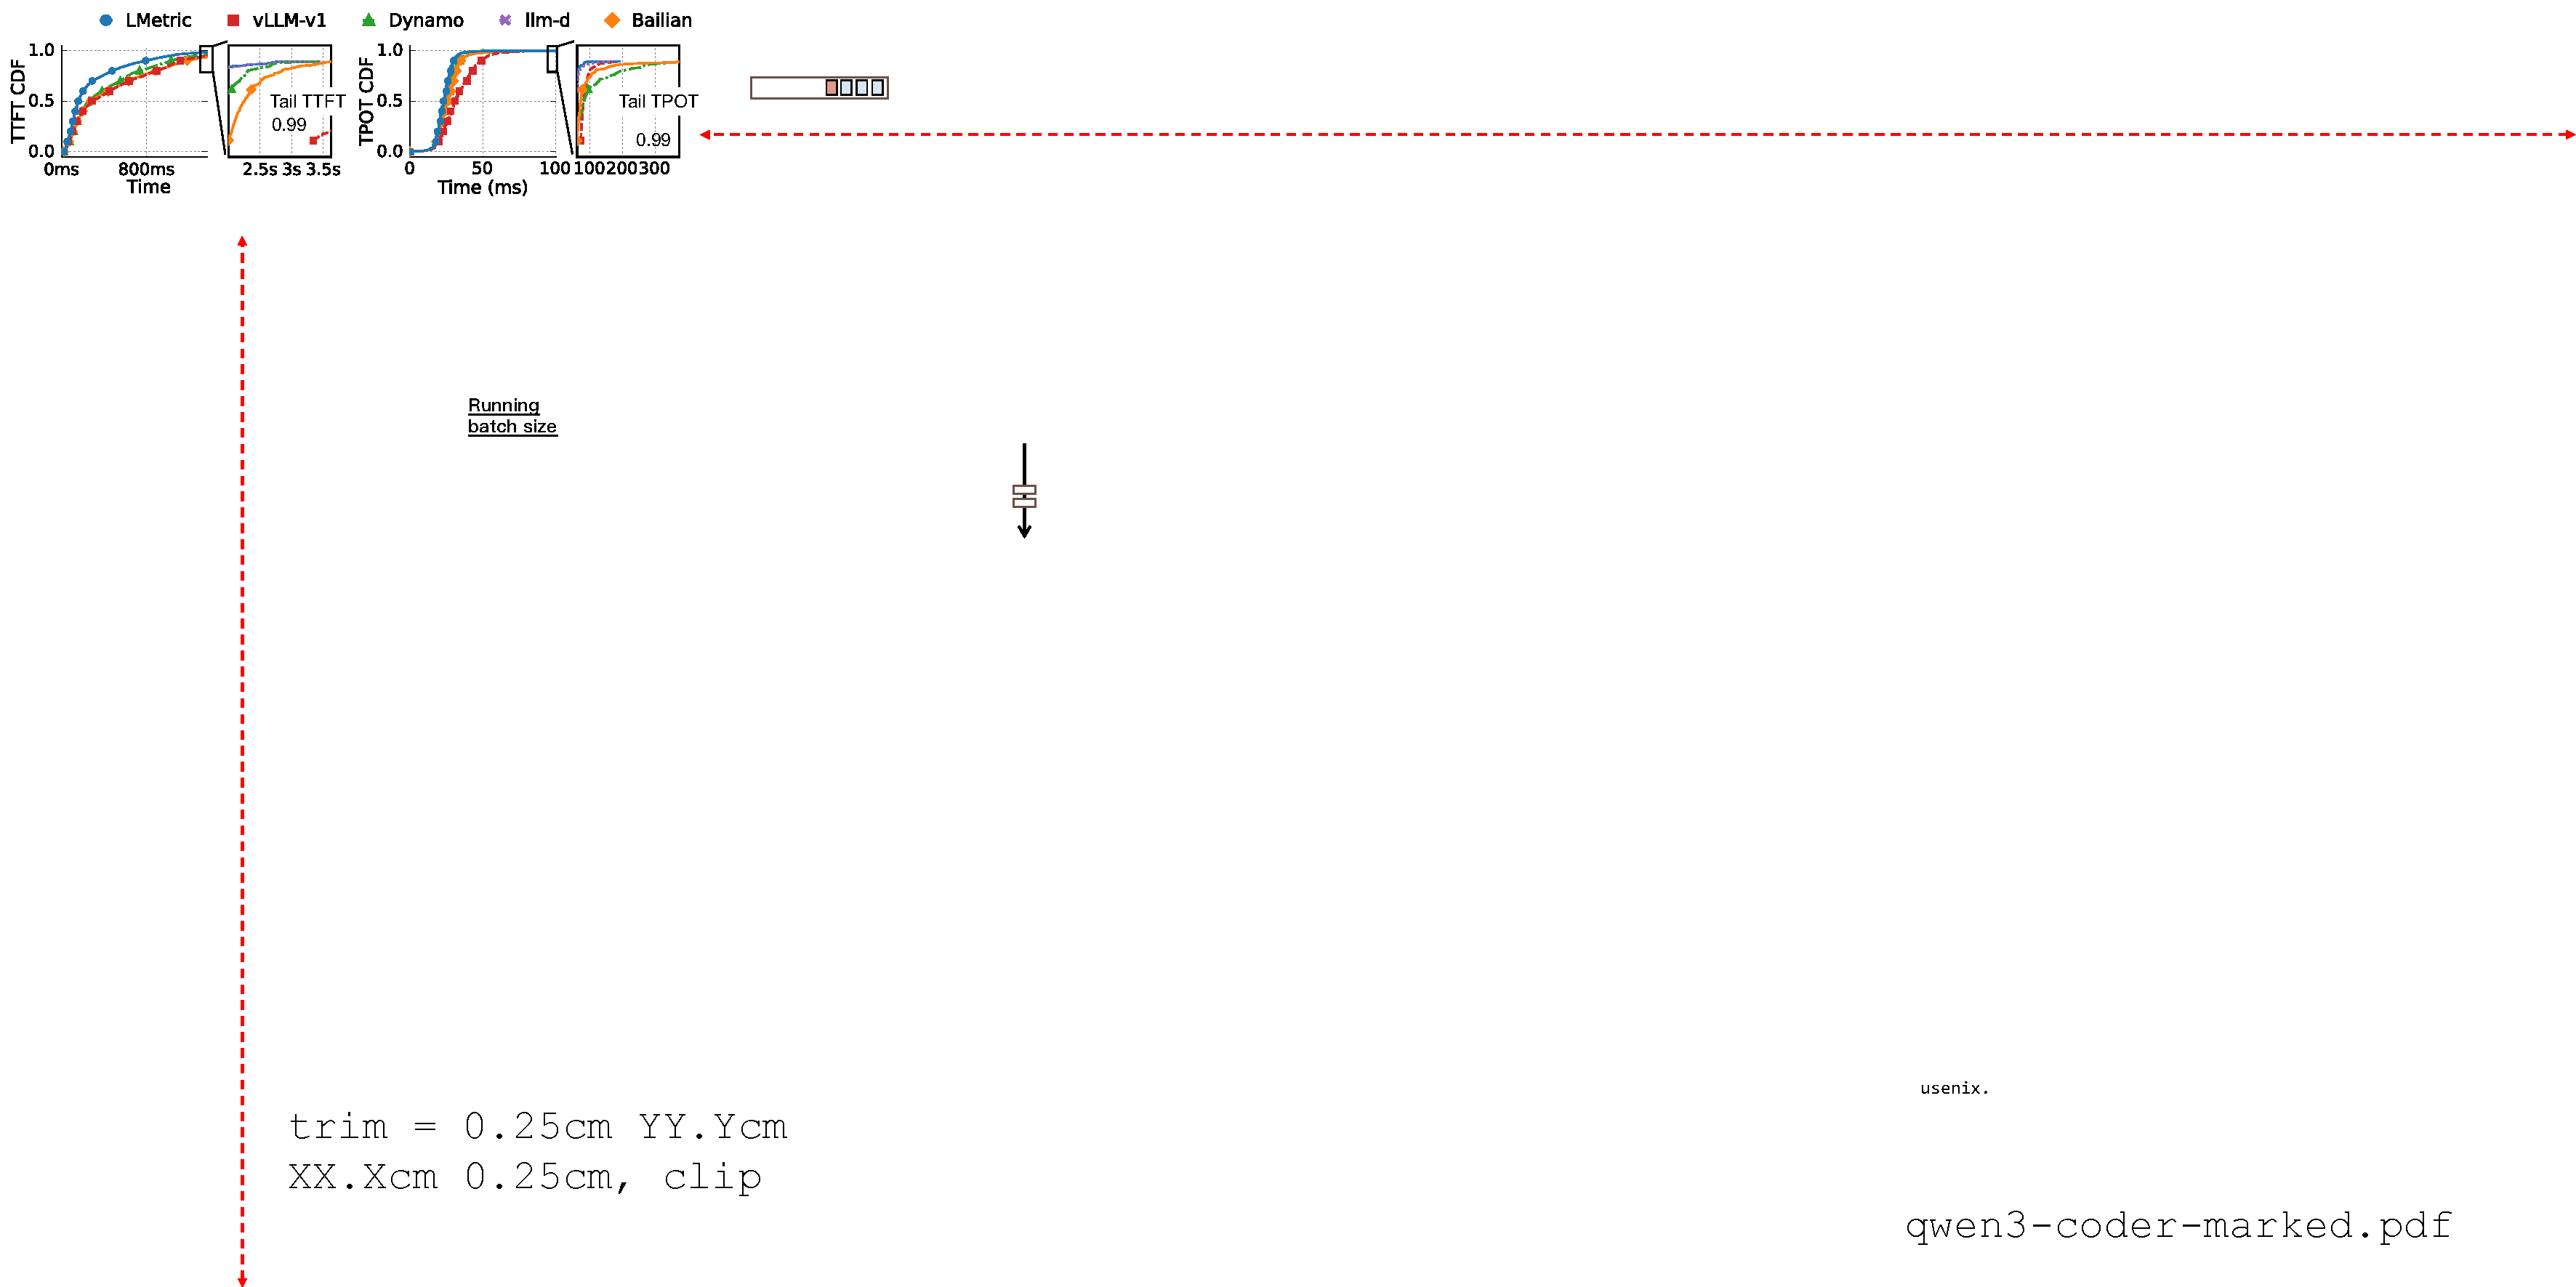
\includegraphics[width=0.98\linewidth, trim=0.25cm 25.2cm 43.75cm 0.25cm, clip]{figs/e2e-cdf-v1/qwen3-coder-marked.pdf}
        \vspace{-8pt}
        \caption{\small{Qwen3-30B on Coder workload.}}
        \label{fig:eval-qwen3-coder}
    \end{subfigure} \\[6pt]
    \begin{subfigure}{\linewidth}
        \centering
        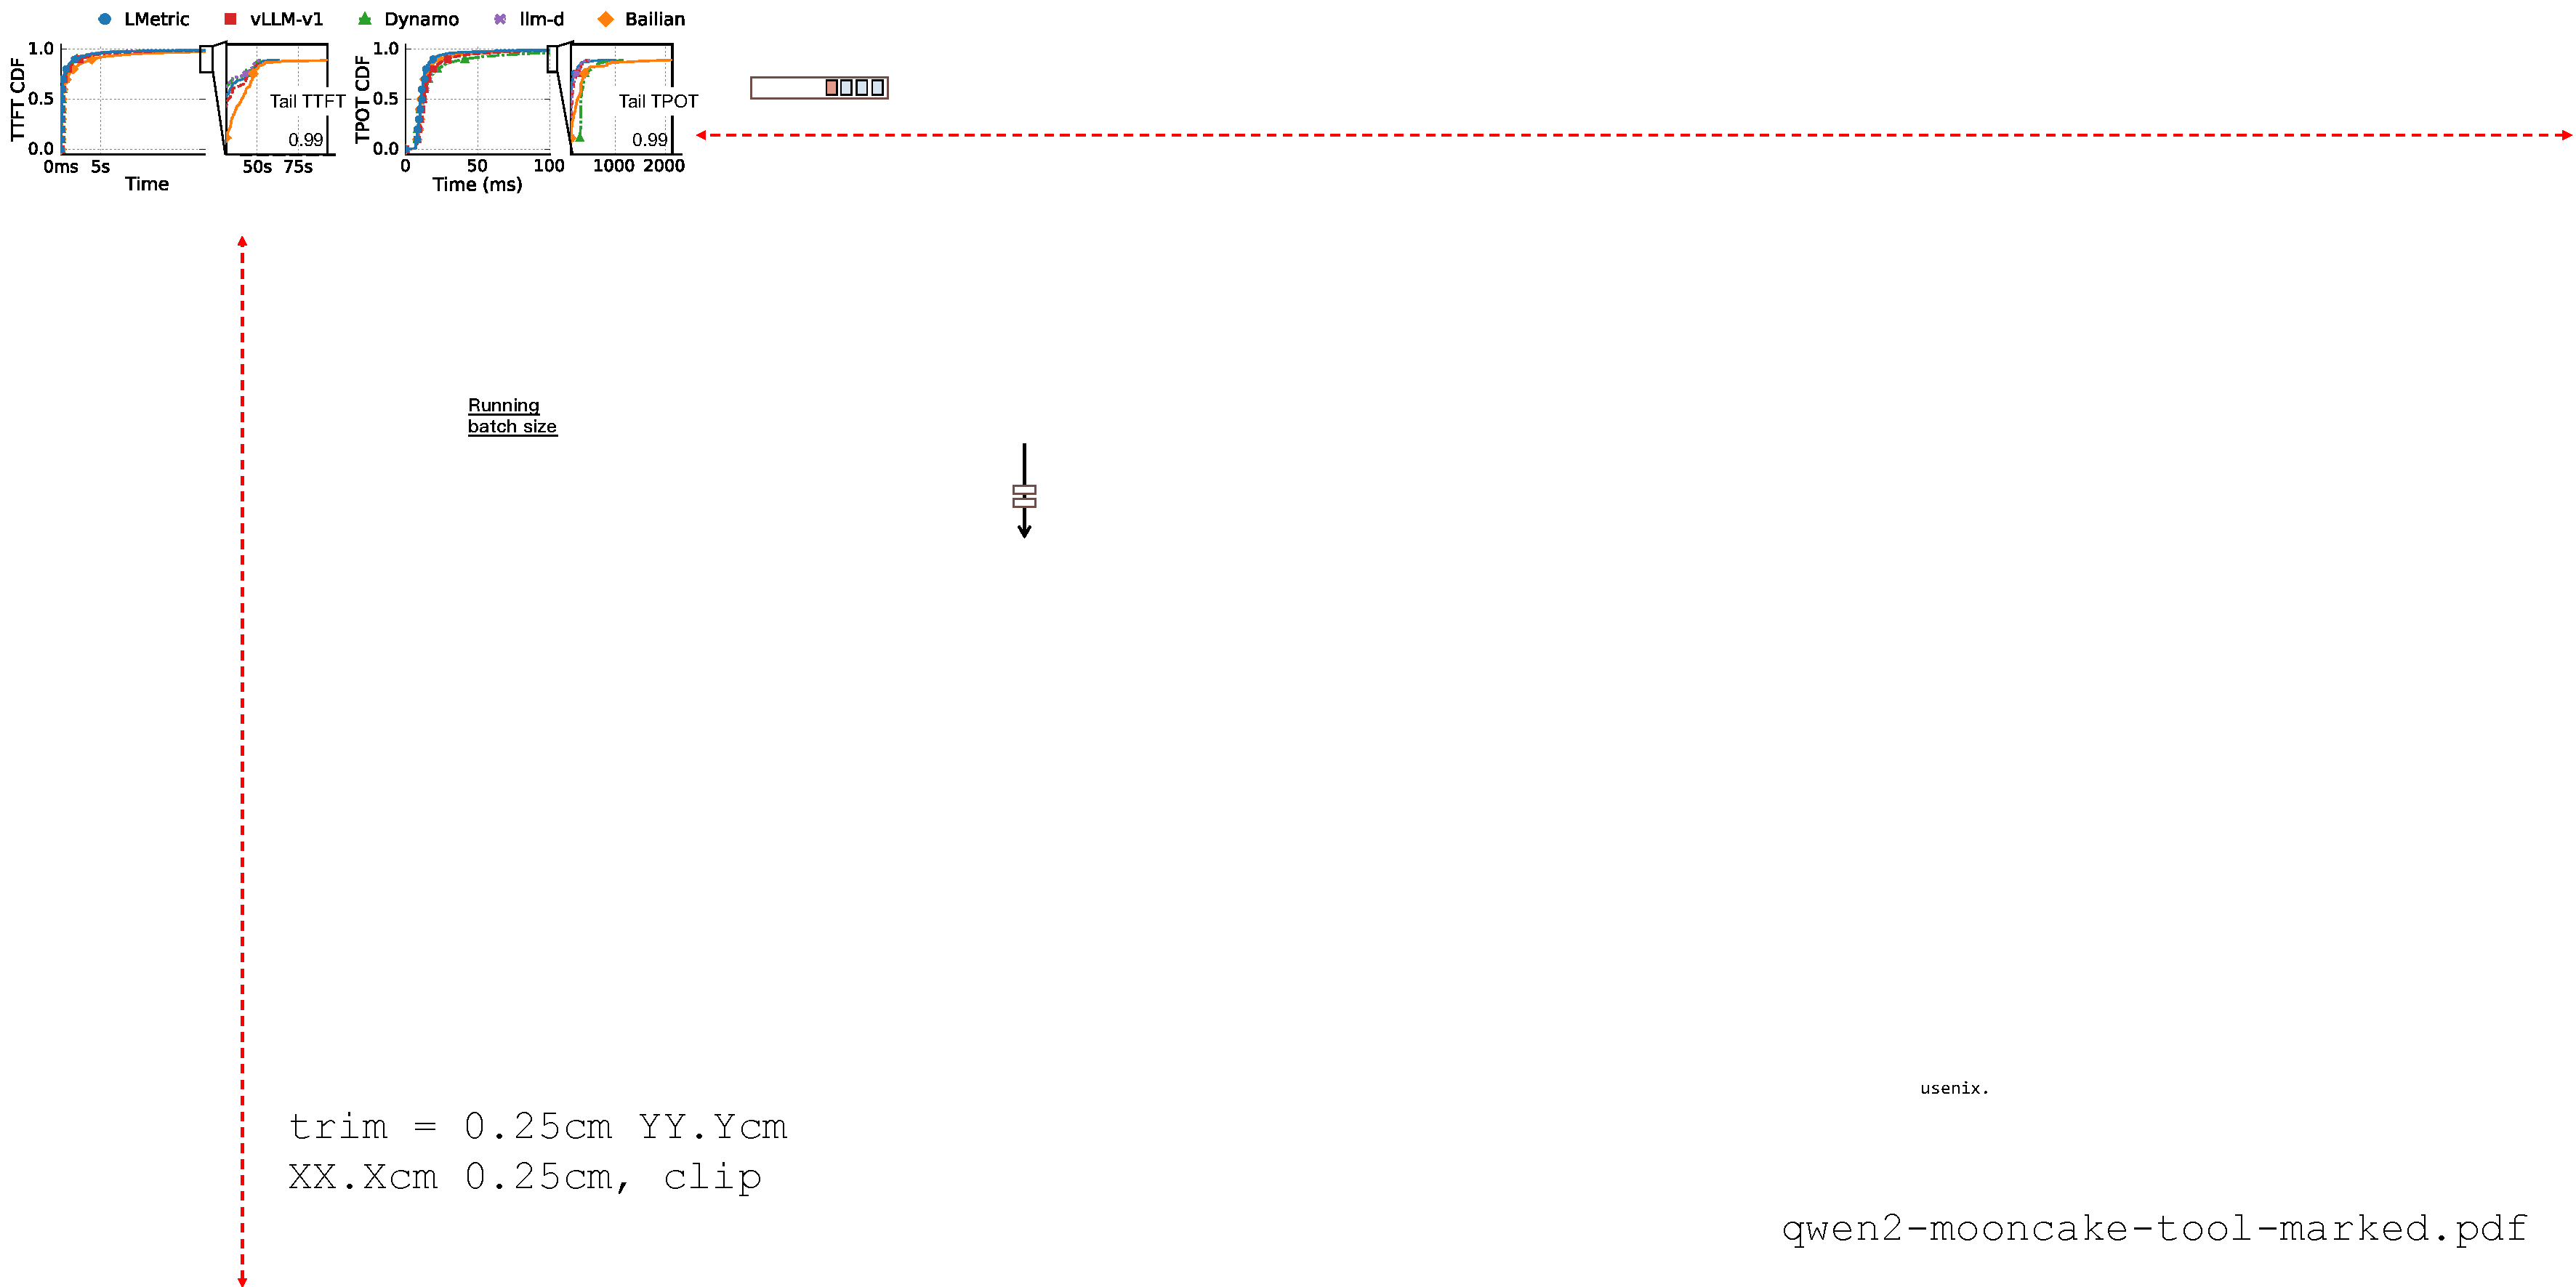
\includegraphics[width=0.98\linewidth, trim=0.25cm 25.2cm 43.75cm 0.25cm, clip]{figs/e2e-cdf-v1/qwen2-mooncake-tool-marked.pdf}
        \vspace{-8pt}
        \caption{\small{Qwen3-30B on Agent (Kimi) workload.}}
        \label{fig:eval-qwen2-mooncake-tool}
    \end{subfigure}
    \caption{\small{End-to-end TTFT and TPOT CDFs of {\sys} and baselines on four workloads.}}
    \label{fig:eval-cdf}
\end{figure}

\begin{figure*}[!t]
    \centering
    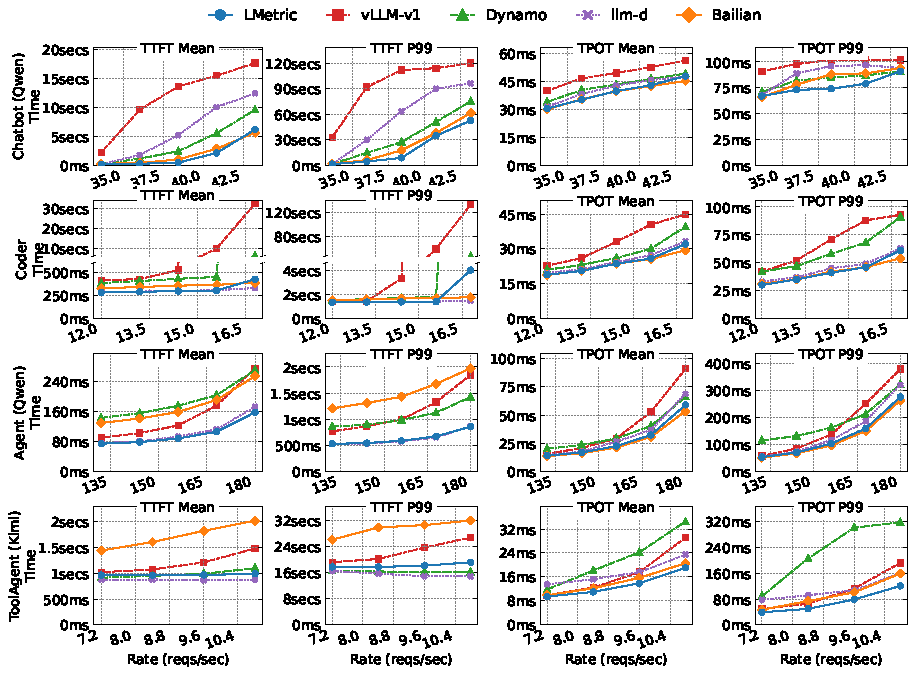
\includegraphics[width=0.9\linewidth]{./figs/scaling-test/scaling-fix-v1.pdf} \\[-3pt]
    \caption{\small{
    End-to-end performance under different request rates. 
    Except the second row that uses a Qwen2-7B model, all other 
    rows use a Qwen3-30B model.
        }}
    \label{fig:scaling-test}
\end{figure*}

\stitle{Baselines. \,}
We compare {\sys} against both open-source schedulers and the current production scheduler used in {\company}.
As some implementations suffer from poor performance due to router implementation issues,
e.g., vLLM exhibits low processing throughput with its Python-based router~\cite{vllm-bug},
we re-implement their policies within our highly optimized Rust router framework described in
\textsection{\ref{sec:factory}}.
For an apples-to-apples comparison,
we compare policies under our framework,
and we have carefully verified that our re-implementations are no slower than their original implementations.
The detailed descriptions of the baselines are as follows:
\\[-15pt]
\begin{itemize}[leftmargin=*,leftmargin=10pt,itemindent=0pt]
\item \textbf{\company} is the production scheduler used in {\company}'s LLM serving system. 
    It adopts a similar linear-combination-based approach as the one shown in {\fig{fig:vllm-kvcache}} (b).
    We have carefully tuned its hyperparameters for each workload to achieve the best performance.
     \\[-15pt]

\item \textbf{vLLM~\cite{vllm-code}} is a widely used LLM serving system that 
    adopts a load-balance only design described in {\fig{fig:vllm-kvcache}} (a).
    
\item \textbf{Dynamo~\cite{ai-Dynamo}} is a popular serving framework
    released by NVIDIA. It also adopts a linear-combination-based approach but with a different
    choice of indicators than {\company}'s.
    The two indicators chosen are the number of prefill tokens (the same as our P-token) for {\kvcache}-awareness
    and the total tokens in the instance for load-balancing awareness.
    The router routes requests to the instance with the minimal regulated and weighted sum of the two indicators.
    Similar to {\company}, we also tune its hyperparameters for each workload for optimal performance. \\[-15pt]

    \item \textbf{llm-d~\cite{llm-d}} adopts a latency-based scheduling policy:
    It estimates the TTFT and routes requests to the instance with the lowest TTFT
    using the simulator-based approach described in {\textsection{\ref{sec:prediction-combination}}}. \\[-15pt]
\end{itemize}

%\noindent
%We don't compare with filter-based approaches as they have shown inferior performance than 
%linear-combination-based approaches,
%as we have extensively discussed in {\textsection{\ref{sec:filter-combination}}}.
%In the following part, we use 16 instances in the scheduling, and scaling the different traces under the SLO constraint.
%\TODO{should put here?}


\stitle{Overall performance. \,}
{\fig{fig:eval-cdf}} shows the end-to-end
TTFT and TPOT CDFs of {\sys} and other baselines on four traces.
All experiments are conducted on a 16-GPU testbed with 16 instances,
and the trace is scaled to half of the maximum load that the testbed can handle.
Due to space constraints, we report results for a representative subset: 
the Qwen3 MoE model on ChatBot, Coder, and Agent workloads, 
and the Qwen2 model on the API workload. 
We observe consistent performance trends across all model--trace combinations. 
% Strategy           Metric       Mean        P50        P95        P99        Min        Max
% ------------------------------------------------------------------------------------------
% CompanyX           TTFT       353.32     112.00    1241.00    3344.72      22.00   28221.00
% CompanyX           TPOT        33.13      27.00      62.00      79.00       0.00     620.00
% Dynamo             TTFT       248.55     136.00     837.00    1452.00      22.00    4004.00
% Dynamo             TPOT        33.99      29.00      60.00      71.00       0.00     345.00
% Mooncake           TTFT       157.84      83.00     578.00    1205.00      23.00    4379.00
% Mooncake           TPOT        31.90      26.00      57.00      77.00       0.00     204.00
% X-Metric           TTFT       166.64      81.00     586.00    1284.52      23.00   15262.00
% X-Metric           TPOT        30.48      25.00      55.00      67.00       0.00     267.00
% vLLM-v1            TTFT      2189.99     112.00   15911.00   32691.85      23.00   69426.00
% vLLM-v1            TPOT        40.14      33.00      76.00      91.00       0.00     318.00

% ====================================================================================================
% X-Metric improvement (%) over other strategies (positive = better, lower latency)
% ----------------------------------------------------------------------------------------------------
% Other Strategy     Mean(TTFT)  P50(TTFT)  P95(TTFT)  P99(TTFT) Mean(TPOT)  P50(TPOT)  P95(TPOT)  P99(TPOT)
% ----------------------------------------------------------------------------------------------------
% CompanyX                52.84      27.68      52.78      61.60       8.00       7.41      11.29      15.19
% Dynamo                  32.95      40.44      29.99      11.53      10.31      13.79       8.33       5.63
% Mooncake                -5.58       2.41      -1.38      -6.60       4.44       3.85       3.51      12.99
% vLLM-v1                 92.39      27.68      96.32      96.07      24.07      24.24      27.63      26.37
% ====================================================================================================
{\sys} outperforms all baselines across all traces.
On the ChatBot workload, 
it reduces the mean TTFT by 92\% and the mean TPOT by 24\% compared to vLLM, 
and it reduces the P99 TPOT by 13\% compared to llm-d---the second best policy---with a similar TTFT.
The improved performance mainly comes from being {\kvcache}-aware
without sacrificing load balancing.
To delve into the behavior of {\sys},
{\fig{fig:eval-e2e-kvcache}} plots the {\kvcache} hit ratio for different systems
on the ChatBot workload.
We can see that {\sys} consistently achieves a {\kvcache} hit ratio comparable to other
{\kvcache}-aware policies, and its ratio is significantly higher than that of the
{\kvcache}-unaware policy (vLLM).
Meanwhile,
{\fig{fig:eval-e2e-imbalance}} further analyzes the imbalance
following the
analysis conducted in \textsection{\ref{sec:challenge-balancing}}.
For ease of presentation, we only compare {\sys} with llm-d---the second-best approach on the ChatBot trace.
We can see that {\sys} achieves a better-balanced load compared to llm-d.

\iffalse
{\fig{fig:eval-qwen3-to-c}} shows the end-to-end TTFT and TPOT of Xmetric and other policies on the ChatBot Trace at Qwen3-30B model.
Xmetric reduces the mean TTFT by 92\%, the mean TPOT by 24\% than vLLM-v1.
Xmetric outperforms other policies in tail latency.
Thanks to the KVCache-aware and Load-balance-aware, Xmetric reduces the P95 TTFT by 96\% than vLLM-v1, P95 TTFT by 27\% than vLLM-v1.
Xmetric improves the P99 TPOT by 13\% than Mooncake, since Xmetric considers the batchsize of each instances.
\fi

% toB
% ==========================================================================================
% Strategy           Metric       Mean        P50        P95        P99        Min        Max
% ------------------------------------------------------------------------------------------
% CompanyX           TTFT       152.13      62.00     614.00    1383.00      13.00    8266.00
% CompanyX           TPOT        13.55      10.00      28.00      69.00       0.00     498.00
% Dynamo             TTFT       120.66      70.00     383.00     688.00      13.00    2063.00
% Dynamo             TPOT        16.57      13.00      37.00      90.00       0.00     494.00
% Mooncake           TTFT        70.55      43.00     209.00     495.00      13.00    2020.00
% Mooncake           TPOT        12.43      11.00      24.00      42.00       0.00     373.00
% X-Metric           TTFT        69.07      41.00     208.00     502.00      13.00    7878.00
% X-Metric           TPOT        11.88      10.00      23.00      40.00       0.00     436.00
% vLLM-v1            TTFT        78.23      44.00     247.00     632.00      14.00    2049.00
% vLLM-v1            TPOT        12.75      11.00      25.00      41.00       0.00     430.00

% ====================================================================================================
% X-Metric improvement (%) over other strategies (positive = better, lower latency)
% ----------------------------------------------------------------------------------------------------
% Other Strategy     Mean(TTFT)  P50(TTFT)  P95(TTFT)  P99(TTFT) Mean(TPOT)  P50(TPOT)  P95(TPOT)  P99(TPOT)
% ----------------------------------------------------------------------------------------------------
% CompanyX                54.60      33.87      66.12      63.70      12.38       0.00      17.86      42.03
% Dynamo                  42.76      41.43      45.69      27.03      28.34      23.08      37.84      55.56
% Mooncake                 2.09       4.65       0.48      -1.41       4.45       9.09       4.17       4.76
% vLLM-v1                 11.71       6.82      15.79      20.57       6.83       9.09       8.00       2.44
% ====================================================================================================

\iffalse
{\fig{fig:eval-qwen2-to-b}} shows the end-to-end TTFT and TPOT of Xmetric and other policies on the API Trace at Qwen2-7B-Instruct model.
Xmetric reduce the mean TTFT by 55\% and mean TPOT by 12\% than the policy used in \company.
\fi

%API Trace reveals the pattern that each requests have very short prompt length and output length.


% Coder
% ==========================================================================================
% Strategy           Metric       Mean        P50        P95        P99        Min        Max
% ------------------------------------------------------------------------------------------
% CompanyX           TTFT       488.96     279.00    1458.00    1996.32      21.00    3620.00
% CompanyX           TPOT        26.95      26.00      39.00      60.00       0.00     374.00
% Dynamo             TTFT       429.56     260.00    1261.00    1698.04      22.00    3430.00
% Dynamo             TPOT        26.13      25.00      37.00      58.00       0.00     396.00
% Mooncake           TTFT       298.88     161.00    1025.00    1373.04      23.00    3447.00
% Mooncake           TPOT        24.29      24.00      33.00      45.00       0.00     170.00
% X-Metric           TTFT       296.41     157.00    1021.00    1374.00      22.00    3439.00
% X-Metric           TPOT        23.61      23.00      32.00      41.00       0.00     189.00
% vLLM-v1            TTFT       524.22     287.00    1346.00    3336.28      21.00   12107.00
% vLLM-v1            TPOT        33.11      31.00      54.00      71.00       0.00     171.00

% ====================================================================================================
% X-Metric improvement (%) over other strategies (positive = better, lower latency)
% ----------------------------------------------------------------------------------------------------
% Other Strategy     Mean(TTFT)  P50(TTFT)  P95(TTFT)  P99(TTFT) Mean(TPOT)  P50(TPOT)  P95(TPOT)  P99(TPOT)
% ----------------------------------------------------------------------------------------------------
% CompanyX                39.38      43.73      29.97      31.17      12.38      11.54      17.95      31.67
% Dynamo                  31.00      39.62      19.03      19.08       9.64       8.00      13.51      29.31
% Mooncake                 0.83       2.48       0.39      -0.07       2.80       4.17       3.03       8.89
% vLLM-v1                 43.46      45.30      24.15      58.82      28.70      25.81      40.74      42.25
% ====================================================================================================

\iffalse
{\fig{fig:eval-qwen3-coder}} shows the end-to-end TTFT and TPOT of Xmetric and other policies on the Coder Trace at Qwen3-30B model.
Xmetric reduce the mean TTFT by 43\% and mean TPOT by 29\% than vLLM.
We can observe that the latency-prediction based policy also performs well in this case. 
This is because that in the Coder scenarios, the LLM frequently reuses the long code prompt given by user and the request number is relatively small.
KVCache hit factors dominates in this scenario.
\fi


% Mooncake tool
% ==========================================================================================
% Strategy           Metric       Mean        P50        P95        P99        Min        Max
% ------------------------------------------------------------------------------------------
% CompanyX           TTFT      1834.23     164.00    8402.10   31006.18      38.00   92987.00
% CompanyX           TPOT        17.57      11.00      41.00     127.02       0.00    2138.00
% Dynamo             TTFT       991.95     166.00    3671.60   16212.58      44.00   52155.00
% Dynamo             TPOT        24.20      12.00      75.15     302.00       0.00    1163.00
% Mooncake           TTFT       866.04     132.00    3403.15   14955.43      40.00   52171.00
% Mooncake           TPOT        17.63      12.00      42.00     108.00       0.00     503.00
% X-Metric           TTFT       968.55     129.00    3780.10   18210.16      35.00   62994.00
% X-Metric           TPOT        13.89      11.00      27.00      79.00       0.00     995.00
% vLLM-v1            TTFT      1213.20     138.00    4772.45   23815.43      34.00   52188.00
% vLLM-v1            TPOT        17.61      12.00      45.00     113.00       0.00     486.00

% ====================================================================================================
% X-Metric improvement (%) over other strategies (positive = better, lower latency)
% ----------------------------------------------------------------------------------------------------
% Other Strategy     Mean(TTFT)  P50(TTFT)  P95(TTFT)  P99(TTFT) Mean(TPOT)  P50(TPOT)  P95(TPOT)  P99(TPOT)
% ----------------------------------------------------------------------------------------------------
% CompanyX                47.20      21.34      55.01      41.27      20.92       0.00      34.15      37.81
% Dynamo                   2.36      22.29      -2.96     -12.32      42.59       8.33      64.07      73.84
% Mooncake               -11.84       2.27     -11.08     -21.76      21.23       8.33      35.71      26.85
% vLLM-v1                 20.17       6.52      20.79      23.54      21.12       8.33      40.00      30.09
% ====================================================================================================

\iffalse
{\fig{fig:eval-qwen2-mooncake-tool}} shows the end-to-end TTFT and TPOT of Xmetric and other policies on the Mooncake Trace at Qwen3-30B model.
Xmetric outperforms other policies in TPOT, reducing 40\% P95 TPOT than vLLM-v1.
The prompt length of the mooncake tool trace is extremely long. So in this case, the latency-based policy outperforms because the accurate predictions
about the prefill cost. 
Xmetrics got the same P50 TTFT with the Mooncake, while suffering from a relatively long tail latency than Mooncake trace because of these extremely long requests.
By splitting this extremely long reequests in some other cluster, we can prevent this issue.
% Xmetric introduces the batchsize factor to reduce the TPOT by 21\% than Mooncake.
% We believe this can improve the experience of our users.

% scale QPS
{\fig{fig:scaling-test}} shows the end-to-end TTFT and TPOT of Xmetric and other policies one different traces and different QPS.
We can see that Xmetric demonstrate stability among different traces and different QPS.



In the ChatBot Trace, Xmetric shows better TTFT and TPOT than any other baselines. 
Xmetric reduces the mean TTFT upto 97\% than vLLM-v1 and mean TPOT upto 27\%.
% how to explain bad mooncake in this case.

In the Coder Trace, Xmetric 


We believe that Xmetric is a simple but effective scheduling policy for LLM scheduling. 
\fi


\begin{figure}[!t]
    %\hspace{-3mm}
    \centering
    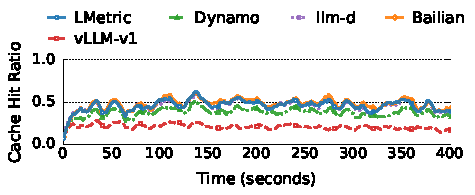
\includegraphics[width=0.98\linewidth]{figs/e2e-kvcache-hit/e2e-kv2.pdf} \\[-0pt]
    \begin{minipage}{1\linewidth}
    \caption{\small{   
        KVCache hit ratio comparison of policies of the Qwen3-30B model on the ChatBot (Qwen) workload.
    }}
    \label{fig:eval-e2e-kvcache}
    \end{minipage} \\[-5pt]
\end{figure} 


\begin{figure}[!t]
    %\hspace{-3mm}
    \centering
    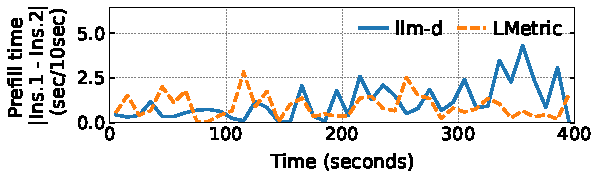
\includegraphics[width=0.98\linewidth]{figs/e2e-kvcache-hit/e2e-lmd-v1.pdf} \\[0pt]
    \begin{minipage}{1\linewidth}
    \caption{\small{   
        A profile of the workload imbalance between two instances under {\sys} and llm-d
        on serving a ChatBot (Qwen) workload with the Qwen3-30B model.
        The reported metric is the absolute served prefill time in each 10-second window
        between the two instances (Inst.).
    }}
    \label{fig:eval-e2e-imbalance}
    \end{minipage} \\[-5pt]
\end{figure} 

\stitle{Performance under different request rates. \,}
{\fig{fig:scaling-test}} further shows how the {\sys} performs under different request arrival rates.
The results are largely consistent with those under a fixed request rate setting:
{\sys} outperforms other baselines across different traces and request rates,
except for the ToolAgent trace,
where {\sys} exhibits a slightly higher (10\%) mean TTFT than llm-d
but achieves a 30\% lower TPOT.
This may be because a simulator-based approach can better estimate
the prefill workload than our simple P-token indicator.
Nevertheless, {\sys} still achieves the lowest TPOT without relying on a complex simulator,
as it considers both {\kvcache} management and (decode) load balancing.
The performance gap between different baselines widens as the request rate increases,
because under high load, a more balanced and {\kvcache}-aware scheduling strategy
can better improve the overall system throughput,
leading to faster consumption of queued requests under high load.

